\subsection{Программный пакет \texttt{NuPropagator}}

\subsubsection{Общее описание и структура}

Пакет \texttt{NuPropagator}~\cite{nupropagator2022} представляет собой модуль для моделирования прохождения потоков нейтрино через вещество, в частности через Землю, с учётом взаимодействий по заряженному и нейтральному токам. Он реализует итеративный метод на основе $\mathcal{Z}$-фактора, что позволяет учитывать регенерацию нейтрино при рассеянии на нуклонах. Пакет написан на языке \texttt{Python3} и поддерживается через платформу \texttt{PyPI}, что обеспечивает его доступность и простоту интеграции в существующие симуляционные цепочки.

\begin{figure}[!h]
\centering
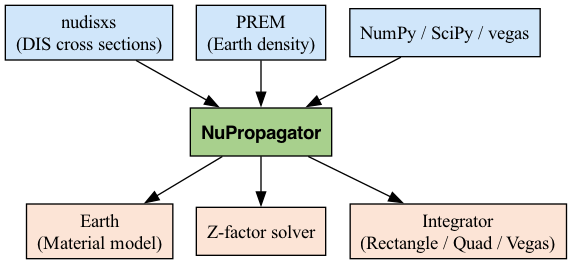
\includegraphics[width=\linewidth]{images/nupropagator_diagram.png}
\caption{Структура программного пакета \texttt{nupropagator} и его зависимости.}
\label{fig:nupropagator1}
\end{figure}

\subsubsection{Физическая модель}

Пакет \texttt{NuPropagator} использует следующие физические компоненты:
\begin{itemize}
  \item модель плотности Земли (PREM);
  \item сечения взаимодействия нейтрино с нуклонами, предоставляемые пакетом \texttt{nudisxs};
  \item итерационный метод Z-фактора для расчёта эволюции нейтринного спектра.
\end{itemize}


\subsubsection{Интеграция с другими модулями}

Пакет \texttt{NuPropagator} может использоваться как самостоятельный инструмент, а также является составной частью общего фреймворка моделирования \texttt{NTSim}, разработанного для нейтринного телескопа Baikal-GVD~\cite{ntsim2025}. 
Он обеспечивает модульную интеграцию с генераторами событий, моделями детектора и другими компонентами цепочки симуляции.

\subsection{Поддержка и установка}

Пакет \texttt{NuPropagator} доступен через \texttt{PyPI} и может быть установлен командой:
\begin{verbatim}
pip install nupropagator
\end{verbatim}
Полная документация доступна на странице проекта, включающей примеры использования и описание API.
